% ============================================================
%  main.tex  —  Rapport ANOVA à mesures répétées (Awa Diaw et Mamady I Bérété)
%  ENSAE – Cours d'Analyse de la Variance
% ============================================================

\documentclass[12pt, a4paper]{report}

% ── Encodage & langue ────────────────────────────────────────
\usepackage[T1]{fontenc}
\usepackage[utf8]{inputenc}
\usepackage[french]{babel}

% ── Mise en page ─────────────────────────────────────────────
\usepackage[top=2.5cm, bottom=2.5cm, left=2.5cm, right=2.5cm]{geometry}
\usepackage{setspace}
\onehalfspacing                     % interligne 1,5

% ── Typographie ──────────────────────────────────────────────
\usepackage{lmodern}
\usepackage{microtype}

% ── Couleurs & graphiques ────────────────────────────────────
\usepackage[dvipsnames, table]{xcolor}
\usepackage{graphicx}
\usepackage{float}
\usepackage{caption}
\usepackage{subcaption}

% ── Tableaux ─────────────────────────────────────────────────
\usepackage{booktabs}
\usepackage{longtable}
\usepackage{array}
\usepackage{multirow}
\usepackage{makecell}
\usepackage{colortbl}

% ── Mathématiques ────────────────────────────────────────────
\usepackage{amsmath, amssymb}

% ── En-têtes & pieds de page ─────────────────────────────────
\usepackage{fancyhdr}
\pagestyle{fancy}
\fancyhf{}
\fancyhead[L]{\small\textit{Étude de l’effet du type de terreau et de la variété sur la croissance de plantes}}
\fancyhead[R]{\small\textit{}}
\fancyfoot[C]{\thepage}
\renewcommand{\headrulewidth}{0.4pt}

% ── Table des matières ───────────────────────────────────────
\usepackage{hyperref}
\hypersetup{
  colorlinks  = true,
  linkcolor   = BrickRed,
  citecolor   = OliveGreen,
  urlcolor    = NavyBlue,
  pdftitle    = {ANOVA à mesures répétées — Croissance des plantes},
  pdfauthor   = {Awa Diaw et Mamady I Bérété},
}
\usepackage{tocloft}

% ── Code R ───────────────────────────────────────────────────
\usepackage{listings}
\definecolor{codebackground}{RGB}{248, 248, 248}
\definecolor{codecomment}{RGB}{100, 100, 100}
\lstset{
  language        = R,
  basicstyle      = \ttfamily\small,
  backgroundcolor = \color{codebackground},
  commentstyle    = \color{codecomment}\itshape,
  keywordstyle    = \color{BrickRed}\bfseries,
  stringstyle     = \color{OliveGreen},
  frame           = single,
  rulecolor       = \color{gray!40},
  breaklines      = true,
  numbers         = left,
  numberstyle     = \tiny\color{gray},
  xleftmargin     = 1.5em,
}

% ── Numérotation des figures/tableaux par chapitre ───────────
\usepackage{chngcntr}
\counterwithin{figure}{chapter}
%\counterwithin{table}{chapter}

% ── Encadrés colorés (page de garde) ────────────────────────
\usepackage{mdframed}

% ── Divers ───────────────────────────────────────────────────
\usepackage{enumitem}
\usepackage{csquotes}
\usepackage[backend=biber, style=apa, sorting=nyt]{biblatex}
\addbibresource{references.bib}

% ============================================================
\begin{document}

% ── PAGE DE GARDE ────────────────────────────────────────────
% (sera rédigée dans page_de_garde.tex)
% ============================================================
%  page_de_garde.tex  —  Page de titre du rapport
% ============================================================

\begin{titlepage}
  \newgeometry{top=2cm, bottom=2cm, left=3cm, right=3cm}
  \centering

  % ════════════════════════════════════════════════
  %  LOGOS (centrés, côte à côte)
  % ════════════════════════════════════════════════
  \vspace*{1cm}

  % ── Logo ANSD ──────────────────────────────────
  
\includegraphics[height=3cm]{figures/logo_ansd.png}\\[0.3cm]
  {\small\bfseries Agence Nationale de la Statistique et de la Démographie}\\[0.1cm]

  \vspace{0.8cm}

  % ── Logo ENSAE ─────────────────────────────────
  
\includegraphics[height=3cm]{figures/logo_ensae.png}\\[0.3cm]
  {\small\bfseries École Nationale de la Statistique et de l'Analyse Économique}\\[0.1cm]

  % ════════════════════════════════════════════════
  %  TITRE
  % ════════════════════════════════════════════════
  \vspace{1.2cm}
  \noindent\rule{0.8\linewidth}{1pt}\\[0.5cm]

  {\LARGE\bfseries Analyse de la variance}\\[0.4cm]
  {\Large\bfseries à mesures répétées}\\[0.3cm]

  \begin{mdframed}[
    linecolor=OliveGreen!70,
    linewidth=0.8pt,
    backgroundcolor=OliveGreen!8,
    innertopmargin=10pt,
    innerbottommargin=10pt,
    innerleftmargin=14pt,
    innerrightmargin=14pt,
    roundcorner=4pt
  ]
    \centering
    {\normalsize\itshape
      Étude de l'effet du type de terreau et de la variété\\[0.2cm]
      sur la croissance de plantes\\[0.3cm]
          }
  \end{mdframed}

  % ════════════════════════════════════════════════
  %  AUTEURE  |  ENCADREUR  (côte à côte)
  % ════════════════════════════════════════════════
  \vspace{1cm}

  \begin{minipage}[t]{0.45\textwidth}
    \centering
    {\small\bfseries Rédigé par :}\\[0.3cm]
    {\normalsize\bfseries Awa Diaw et Mamady I Bérété}\\[0.15cm]
    {\small Élèves en ISE2}
  \end{minipage}
  \hfill
  \begin{minipage}[t]{0.45\textwidth}
    \centering
    {\small\bfseries Chargé du cours :}\\[0.3cm]
    {\normalsize\bfseries M. Carlos Akakpovi}\\[0.15cm]
    {\small  Ingénieur statisticien économiste}
  \end{minipage}

  % ════════════════════════════════════════════════
  %  ANNÉE ACADÉMIQUE
  % ════════════════════════════════════════════════
  \vfill

  {\small Année académique \textbf{2025--2026} \quad|\quad Mars 2026}\\[0.2cm]

  \restoregeometry
\end{titlepage}
\thispagestyle{empty}
\cleardoublepage

% ── NUMÉROTATION ROMAINE pour les pages liminaires ───────────
\pagenumbering{roman}
\setcounter{page}{1}

% ── AVANT-PROPOS ────────────────────────────────────────────
\chapter*{Avant-propos}
\addcontentsline{toc}{chapter}{Avant-propos}

L'École nationale de la Statistique et de l'Analyse économique Pierre Ndiaye de Dakar (ENSAE) a pour mission de
former des ingénieurs capables de combiner solides connaissances théoriques et expérience
pratique. La rédaction de ce rapport s'inscrit dans le cadre du cours d'Analyse de la
Variance, qui constitue un outil privilégié pour l'application des méthodes statistiques à
des données expérimentales.

Le présent travail se concentre sur l'analyse de la croissance de plantes en fonction de
différents types de terreau et de variétés, à l'aide d'une ANOVA à mesures répétées.
L'objectif n'est pas seulement descriptif : il s'agit d'identifier les facteurs influençant
significativement la variable étudiée et leurs interactions.

Nous tenons à remercier M.\ Carlos Akakpovi, chargé du cours, pour ses
conseils et sa disponibilité tout au long de ce projet.

  \vspace{0.8cm}
Les scripts R utilisés pour l'ensemble des analyses (importation, nettoyage, descriptif,
ANOVA, LMM, graphiques) sont disponibles à l'adresse suivante :
\begin{center}
  \url{https://github.com/awa-d/projet_anova2026}
\end{center}


  \vspace{0.8cm}
Les éventuelles erreurs et interprétations restent la responsabilité des auteurs.
\clearpage

% ── TABLE DES MATIÈRES ───────────────────────────────────────
\tableofcontents
\clearpage

% ── LISTE DES FIGURES ────────────────────────────────────────
\listoffigures
\addcontentsline{toc}{chapter}{Liste des figures}

% ── LISTE DES TABLEAUX ───────────────────────────────────────
%\listoftables
%\addcontentsline{toc}{chapter}{Liste des tableaux}
%\clearpage



% ============================================================
%  CORPS DU RAPPORT
% ============================================================
% ── Résumé─────────────────────────────────────────────
\chapter*{Résumé}
\addcontentsline{toc}{chapter}{Résumé}


Ce rapport analyse l'effet du \textbf{type de terreau} (Manguier, Caïlcédrat, Anacarde) et
de la \textbf{variété} (Var1, Var2) sur la croissance de plantes, mesurée par la hauteur à
quatre répétitions successives. Le dispositif expérimental, constitué de 96 sujets avec
mesures répétées, justifie l'utilisation d'une \textbf{ANOVA à mesures répétées} et d'un
\textbf{modèle linéaire mixte}.

\vspace{0.4cm}

\noindent
L'analyse descriptive (statistiques univariées, bivariées, ACP) révèle des trajectoires de
croissance non parallèles entre variétés et une hétérogénéité entre répétitions. L'analyse
inférentielle montre que la \textbf{variété} et la \textbf{répétition} influencent
significativement la hauteur des plantes, et que leur \textbf{interaction est significative}
($p < 0{,}001$). Le type de terreau, en revanche, n'a pas d'effet significatif ($p = 0{,}303$).
Les tests post-hoc (Bonferroni) confirment que la différence entre variétés est marquée à la
première répétition puis s'efface progressivement.

\vspace{1cm}

\textbf{Mots-clefs : }

\noindent
ANOVA à mesures répétées \textbullet{} ACP \textbullet{} Interaction\textbullet{} Modèle linéaire mixte \textbullet{} Sphéricité \textbullet{} Terreau \textbullet{} Test de Bonferroni \textbullet{}Variété

% ── INTRODUCTION ─────────────────────────────────────────────
\chapter*{Introduction}
\addcontentsline{toc}{chapter}{Introduction}

La croissance des plantes dépend de multiples facteurs, notamment les caractéristiques du
substrat de culture et les propriétés génétiques des variétés végétales. Le type de terreau
influence la disponibilité des nutriments, la rétention en eau et l'aération des racines,
tandis que la variété conditionne le potentiel de croissance et la réponse aux conditions de
culture. L'analyse conjointe de ces facteurs est essentielle pour identifier les combinaisons
favorables à une croissance optimale des plantes.

La présente étude s'appuie sur des données issues d'une expérimentation agronomique portant
sur trois types de terreau (manguier, caïlcédrat et anacardier) appliqués à deux variétés de
plantes (Var1 et Var2). L'expérience a été répétée à quatre reprises, avec des mesures
successives de la hauteur des plantes. Ce dispositif expérimental conduit à des observations
dépendantes dans le temps, ce qui justifie le recours à des méthodes statistiques adaptées
aux mesures répétées.

L’objectif est de voir s’il existe une association type de terreau et type de variété qui favorise la croissance des plantes. Plus précisément, l'étude cherche à déterminer : (i) si le type de terreau influence significativement la
hauteur des plantes, (ii) si la variété a un effet propre sur la croissance, et (iii) si
l'évolution de la croissance au fil des répétitions dépend des combinaisons terreau–variété.

Le rapport est organisé comme suit. La première partie présente une revue synthétique de la
littérature et le cadre théorique relatif à l'ANOVA à mesures répétées. La deuxième partie
est consacrée à l'analyse descriptive des données. La troisième partie présente l'analyse
inférentielle suivie de l'interprétation des résultats. Enfin, une conclusion générale
discute les principaux enseignements, les limites et les perspectives de recherche.


% ── NUMÉROTATION ARABE pour le corps du rapport ──────────────
\pagenumbering{arabic}
\setcounter{page}{1}

% ============================================================
\chapter{Revue de littérature et cadre théorique}
% ============================================================

\section{Revue de la littérature (théorique et empirique)}

L’analyse de la variance (ANOVA) constitue un cadre statistique central pour l’étude des effets de traitements dans les dispositifs expérimentaux, notamment en agronomie et en biostatistique. Introduite par Ronald Fisher (1935), elle repose sur la décomposition de la variabilité totale d’une variable en composantes attribuables aux facteurs étudiés et à l’erreur aléatoire, permettant la comparaison simultanée de plusieurs moyennes dans un cadre probabiliste rigoureux.

En agronomie, l’ANOVA est largement mobilisée pour évaluer l’effet de pratiques culturales (type de sol, amendements, fertilisation) sur la croissance des cultures. Les travaux de Douglas Montgomery (2017) montrent que les plans factoriels constituent un outil méthodologique central pour analyser simultanément plusieurs facteurs explicatifs et leurs interactions. Ces interactions sont essentielles, car l’effet d’un traitement (par exemple un type de terreau) peut dépendre de la variété végétale considérée.

De nombreuses études biologiques reposent sur des mesures répétées dans le temps sur les mêmes individus. Dans ce contexte longitudinal, l’application de méthodes conçues pour des échantillons indépendants conduit à une mauvaise estimation de la variance résiduelle et à une inflation du risque d’erreur de type I (David Howell, 2013). L’ANOVA à mesures répétées permet de tenir compte de la dépendance intra-individuelle en distinguant la variabilité inter-individus de la variabilité intra-individus au cours du temps.

Dans les dispositifs combinant plusieurs facteurs inter-individus (par exemple le type de terreau et la variété) et un facteur intra-individu (le temps), on parle de plans mixtes. Andy Field (2012) met en évidence l’intérêt de ces modèles pour analyser simultanément les effets principaux et les interactions avec le temps, ce qui est particulièrement pertinent pour l’étude des dynamiques de croissance végétale.

Sur le plan méthodologique, l’ANOVA à mesures répétées repose sur plusieurs hypothèses, notamment la normalité des résidus, l’homogénéité des variances et la sphéricité. La violation de la sphéricité entraîne une inflation de la statistique de test F et, par conséquent, du risque de faux positifs ; des corrections des degrés de liberté (Greenhouse–Geisser, Huynh–Feldt) sont alors recommandées (**Andy Field, 2012 ; David Howell, 2013).

Enfin, la littérature souligne l’importance d’une phase exploratoire préalable à toute analyse inférentielle. L’analyse exploratoire des données proposée par John Tukey (1977) permet de comprendre la structure des données et de détecter d’éventuelles anomalies. Dans le cas de mesures répétées, l’Analyse en Composantes Principales (ACP) proposée par Ian Jolliffe (2002) fournit une représentation synthétique des profils de croissance et complète utilement l’ANOVA à mesures répétées dans l’interprétation des résultats.

En synthèse, la littérature met en évidence l’intérêt de combiner une exploration descriptive des données et une modélisation inférentielle adaptée aux dispositifs longitudinaux. L’ANOVA à mesures répétées apparaît ainsi comme un outil pertinent pour analyser l’effet conjoint du type de terreau, de la variété et du temps sur la croissance des plants.

\section{Présentation succincte de l'Analyse de la Variance (ANOVA)}

L'Analyse de la Variance (ANOVA) est une méthode statistique inférentielle permettant de
comparer les moyennes de plusieurs groupes et d'évaluer l'effet de facteurs explicatifs
qualitatifs sur une variable quantitative. Contrairement aux comparaisons multiples de
moyennes par tests $t$, l'ANOVA permet de contrôler le risque global d'erreur de type~I en
testant simultanément l'égalité de plusieurs moyennes.

Dans sa forme générale, l'ANOVA repose sur la décomposition de la variabilité totale de la
variable étudiée en une composante expliquée par les facteurs (variabilité inter-groupes) et
une composante résiduelle (variabilité intra-groupes). Le test de Fisher (statistique~$F$)
évalue si la variabilité expliquée par le modèle est significativement supérieure à la
variabilité résiduelle.

On distingue notamment :
\begin{itemize}[leftmargin=*, label=\textbullet]
  \item l'ANOVA à un facteur (un seul facteur explicatif) ;
  \item l'ANOVA à deux facteurs ou plus, avec ou sans interaction, permettant d'étudier
        non seulement les effets propres de chaque facteur, mais aussi leurs effets combinés ;
  \item les extensions de l'ANOVA aux plans expérimentaux plus complexes (plans équilibrés
        ou non, données corrélées, mesures répétées).
\end{itemize}

\section{Présentation succincte de l'ANOVA à mesures répétées : principe, hypothèses et utilité}

L'ANOVA à mesures répétées constitue une extension de l'ANOVA classique adaptée aux
situations où plusieurs mesures sont réalisées sur les mêmes unités statistiques au cours du
temps ou sous différentes conditions. Dans ce contexte, l'hypothèse d'indépendance des
observations n'est plus vérifiée, car les mesures successives effectuées sur une même unité
sont corrélées.

Le principe est de modéliser explicitement cette dépendance intra-individuelle en
distinguant : la variabilité inter-individus (différences entre plantes), la variabilité
intra-individus (évolution des mesures pour une même plante au fil des répétitions), et les
effets des facteurs expérimentaux ainsi que leurs interactions avec le facteur temps.

Cette approche présente plusieurs avantages : (i)~elle augmente la puissance statistique en
contrôlant la variabilité propre à chaque individu ; (ii)~elle permet d'analyser l'évolution
de la réponse dans le temps ; (iii)~elle autorise l'étude d'interactions entre facteurs fixes
et facteur de répétition.

L'ANOVA à mesures répétées repose sur trois hypothèses principales :

\begin{itemize}[leftmargin=*, label=\textbullet]
  \item \textbf{Normalité des résidus :} les résidus du modèle sont supposés suivre
        approximativement une loi normale, principalement requise pour la validité des tests
        de significativité.
  \item \textbf{Homogénéité des variances :} la variance de la variable réponse doit être
        comparable entre les groupes définis par les facteurs (terreau, variété).
  \item \textbf{Sphéricité :} hypothèse spécifique aux mesures répétées, selon laquelle les
        variances des différences entre toutes les paires de niveaux du facteur de répétition
        sont égales. Sa violation peut conduire à une inflation du risque d'erreur de type~I,
        corrigée via les corrections de Greenhouse–Geisser ou de Huynh–Feldt.
\end{itemize}

Lorsque certaines hypothèses sont fortement violées, les modèles linéaires mixtes constituent
une alternative plus flexible, permettant de modéliser la structure de corrélation entre
mesures répétées et d'intégrer des effets aléatoires associés aux individus.

% ============================================================
\chapter{Analyse descriptive}
% ============================================================

\section{Description de la base de données et du dispositif expérimental}

Les données analysées proviennent d'une expérimentation biologique réelle visant à étudier
l'effet du type de terreau et de la variété de plante sur la croissance végétative, mesurée
par la hauteur des plants. La base comprend \textbf{96 sujets} (plantes), avec pour chaque
observation : l'identifiant du sujet, le type de terreau, la variété, la répétition et la
hauteur mesurée, comme l'illustre ce tableau ~\ref{tab:explo}
\begin{figure}[H]
  \centering
  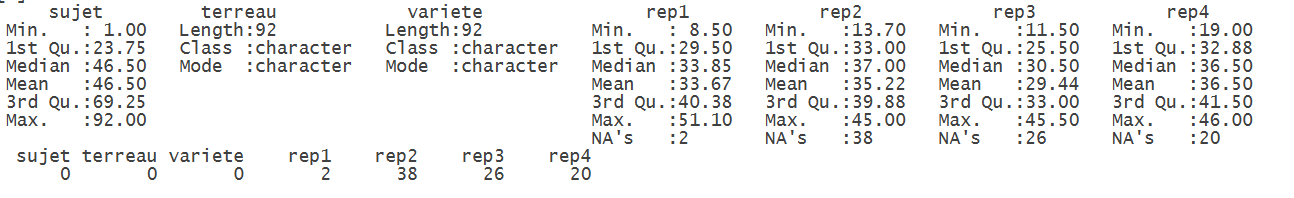
\includegraphics[width=0.85\textwidth]{figures/tableau_explo.png}
  \caption{Exploration de la base de données}
  \label{tab:explo}
\end{figure}
Le dispositif est structuré autour de :
\begin{itemize}[leftmargin=*, label=\textbullet]
  \item \textbf{Facteur 1 — Type de terreau} (3 modalités) : Manguier (Ma), Caïlcédrat (Ca),
        Anacarde (An) ;
  \item \textbf{Facteur 2 — Variété} (2 modalités) : Var1, Var2 ;
  \item \textbf{Facteur intra-sujet — Répétition} (4 modalités) : rep1 à rep4 ;
  \item \textbf{Variable dépendante} : hauteur des plantes (cm), mesurée à chaque répétition.
\end{itemize}

Ce dispositif correspond à un plan factoriel croisé à deux facteurs fixes (terreau $\times$
variété) avec un facteur intra-sujet (répétition), justifiant l'utilisation d'une ANOVA à
mesures répétées et, en complément, d'un modèle linéaire mixte.

\section{Statistiques descriptives univariées}

Le Tableau~\ref{tab:desc_univ} présente les statistiques descriptives des variables
principales. La hauteur moyenne des plants est de 33,7~cm (écart-type 8,1~cm), avec une
médiane proche (34,4~cm), indiquant une distribution globalement symétrique. Les plants sont
répartis presque équitablement entre les variétés Var1 (51\%) et Var2 (49\%). Concernant le
type de terreau, les effectifs sont légèrement déséquilibrés : Ca~(37\%), Ma~(37\%),
An~(26\%). La distribution des mesures selon les répétitions est homogène, ce qui permet de
tester l'effet du temps dans les analyses de mesures répétées. Le tableau inclut 86 valeurs
manquantes, conservées afin de ne pas perdre d'information.

% ── Insérer ici le tableau généré par R/gtsummary ────────────
\begin{figure}[H]
  \centering
  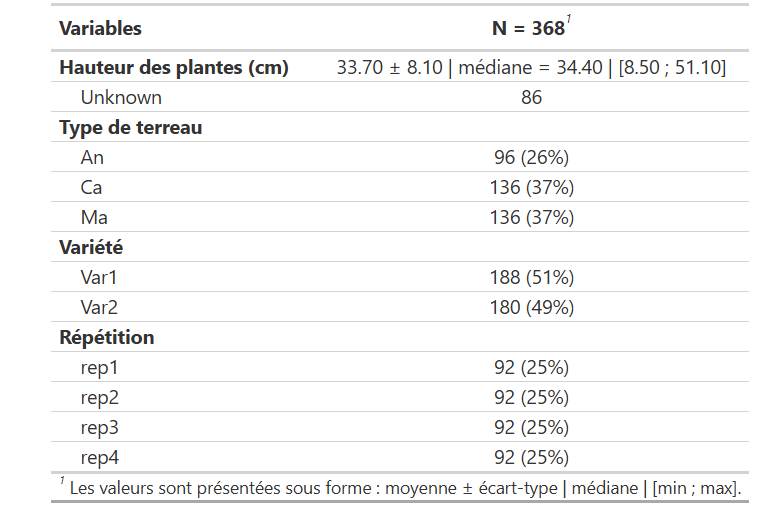
\includegraphics[width=0.85\textwidth]{figures/tableau_desc_univ.png}
  \caption{Statistiques descriptives des plants selon les traitements.}
  \label{tab:desc_univ}
\end{figure}

La distribution globale de la hauteur (Figure~\ref{fig:histo}) montre une distribution
étalée à gauche et quelques valeurs extrêmes, avec une concentration autour de 34–36~cm.

\begin{figure}[H]
  \centering
  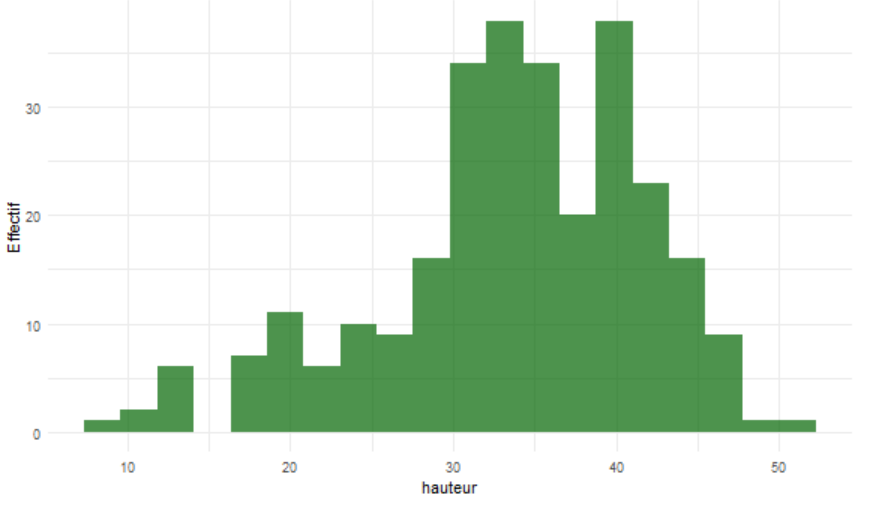
\includegraphics[width=0.75\textwidth]{figures/histo_hauteur.png}
  \caption{Distribution globale de la hauteur des plantes.}
  \label{fig:histo}
\end{figure}

\section{Statistiques descriptives bivariées}

La Figure~\ref{fig:boxplot_rep} présente les boxplots de la hauteur par type de terreau et
par variété, déclinés selon la répétition. Les hauteurs ne sont pas constantes d'une
répétition à l'autre : la position des médianes et l'étendue des boîtes varient au fil du
temps, suggérant une évolution des mesures entre rep1 et rep4. Les valeurs atypiques
visibles reflètent la variabilité réelle et le faible effectif par sous-groupe ; la
winsorisation (1\%–99\%) a été appliquée au niveau terreau $\times$ variété.

\begin{figure}[H]
  \centering
  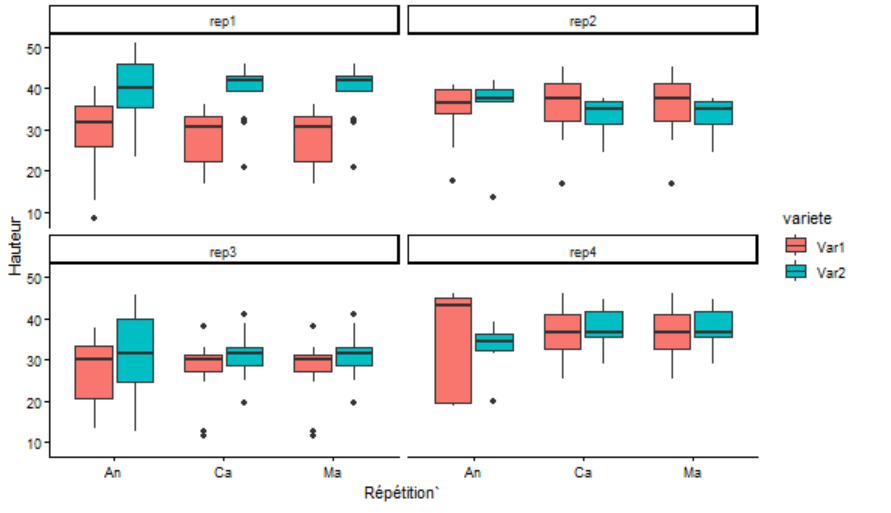
\includegraphics[width=\textwidth]{figures/boxplot_hauteur_repet.png}
  \caption{Boxplots de la hauteur par type de terreau et variété pour chaque répétition.}
  \label{fig:boxplot_rep}
\end{figure}

Les courbes de croissance (Figure~\ref{fig:courbes}) montrent que la hauteur des plants varie
selon la répétition, avec une baisse autour de rep3. Les trajectoires des deux variétés ne
sont pas parallèles — l'écart entre Var1 et Var2 change au fil du temps — ce qui suggère une
interaction possible variété $\times$ répétition. Les profils sont globalement similaires
entre les trois types de terreau, indiquant un effet visuel modéré du terreau.

\begin{figure}[H]
  \centering
  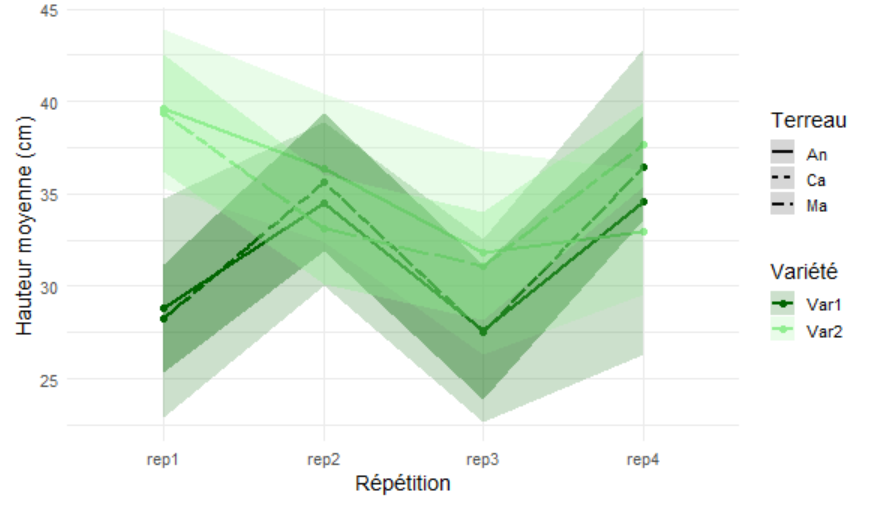
\includegraphics[width=\textwidth]{figures/courbes_croissance.png}
  \caption{Courbes de croissance des plants par répétition (intervalle de confiance à 95\%).}
  \label{fig:courbes}
\end{figure}

\section{Analyse exploratoire multivariée (ACP)}

L'Analyse en Composantes Principales (ACP) est utilisée ici comme outil exploratoire
complémentaire à l'ANOVA, afin de synthétiser les profils de croissance avant les tests
formels. Les données manquantes ont été imputées par la méthode \texttt{imputePCA} (package
\textit{missMDA}).

Les deux premières composantes expliquent \textbf{64,5\%} de la variance totale
(Figure~\ref{fig:screeplot}). La projection des individus selon le type de terreau
(Figure~\ref{fig:acp_ind}) ne met pas en évidence de séparation nette entre les groupes,
indiquant une forte variabilité intra-terreau. Le cercle des corrélations
(Figure~\ref{fig:acp_var}) révèle des profils différenciés entre rep1 et rep4 : rep1 et rep3
sont corrélées, tandis que rep2 et rep4 s'opposent sur la première composante. Ces résultats
suggèrent une hétérogénéité entre répétitions, justifiant la prise en compte de l'effet
répétition dans l'analyse inférentielle.

\begin{figure}[H]
  \centering
  \begin{subfigure}[b]{0.48\textwidth}
    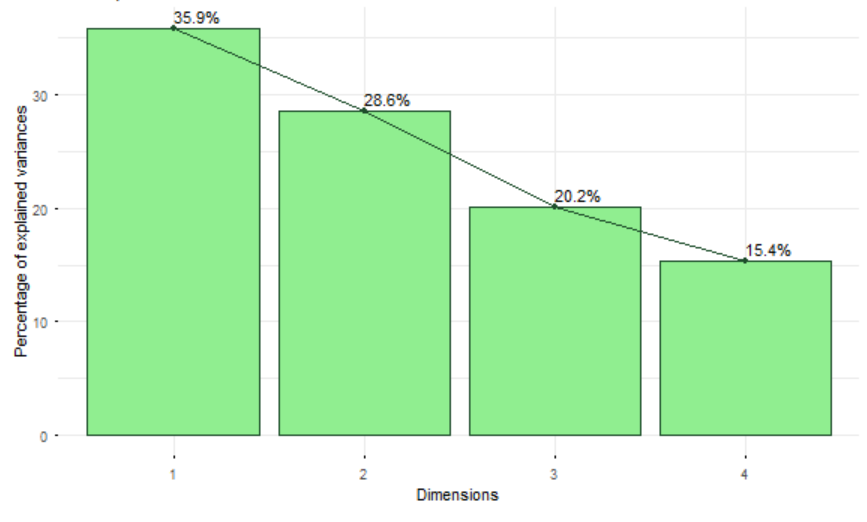
\includegraphics[width=\textwidth]{figures/acp_screeplot.png}
    \caption{Scree plot — variance expliquée.}
    \label{fig:screeplot}
  \end{subfigure}
  \hfill
  \begin{subfigure}[b]{0.48\textwidth}
    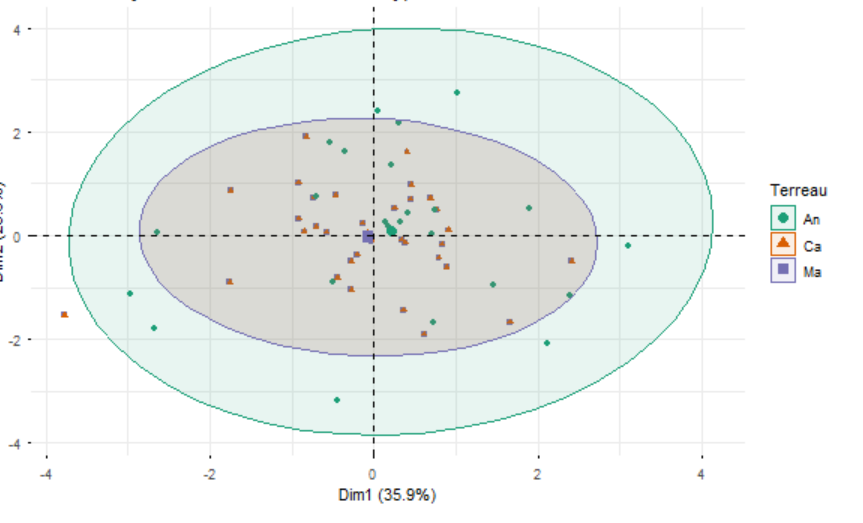
\includegraphics[width=\textwidth]{figures/acp_individus.png}
    \caption{Projection des individus selon le terreau.}
    \label{fig:acp_ind}
  \end{subfigure}
  \vspace{0.5cm}
  \begin{subfigure}[b]{0.48\textwidth}
    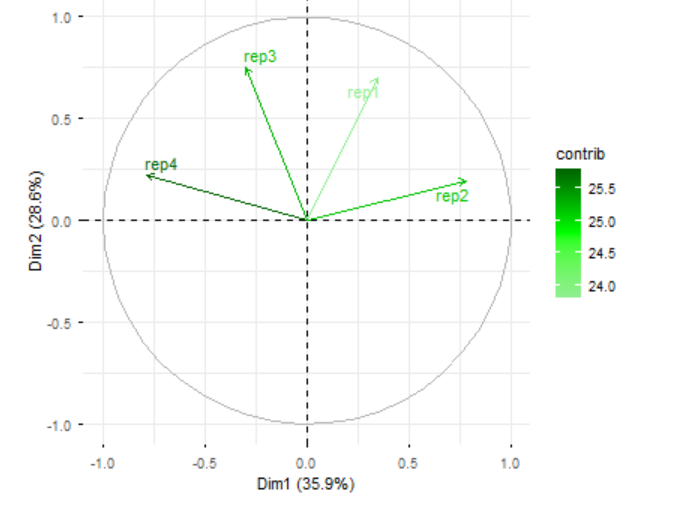
\includegraphics[width=\textwidth]{figures/acp_variables.png}
    \caption{Cercle des corrélations (rep1–rep4).}
    \label{fig:acp_var}
  \end{subfigure}
  \caption{Résultats de l'ACP sur les données de croissance.}
\end{figure}

% ============================================================
\chapter{Analyse inférentielle}
% ============================================================

Cette section vise à étudier l'effet des facteurs \textbf{terreau} et \textbf{variété} sur
la \textbf{hauteur des plantes} au fil des \textbf{répétitions}, à l'aide d'une ANOVA à
mesures répétées et d'un modèle linéaire mixte (LMM).

\section{Types d'ANOVA et choix du modèle}

Avant de lancer l'analyse, il convient de choisir le modèle adapté à la structure des
données : mesures répétées, facteurs inter- et intra-sujets, présence de valeurs manquantes.

Le \textbf{modèle linéaire mixte} est retenu pour tenir compte de la variabilité individuelle
et des valeurs manquantes. Il sera comparé à l'ANOVA mixte (split-plot) afin d'évaluer l'impact de la
gestion des NA sur les résultats.

\section{Vérification des hypothèses}

\subsection*{Valeurs extrêmes}
Les valeurs aberrantes ont d’abord été recherchées au sein de groupes homogènes définis par la combinaison du terreau, de la variété et de la répétition. Cette approche vise, en principe, à comparer des plantes soumises aux mêmes conditions expérimentales au même moment. Cependant, ce niveau de croisement conduit à des effectifs très faibles par groupe (parfois une ou deux observations seulement), rendant la règle de l’écart interquartile (IQR) instable. Dans ce contexte, l’ensemble des observations a été artificiellement identifié comme valeur aberrante, ce qui invalide cette approche pour ce jeu de données.

En conséquence, la détection des valeurs extrêmes a été réalisée par combinaison du terreau et de la variété, ce qui permet de constituer des groupes biologiquement cohérents tout en garantissant des effectifs suffisants pour une application pertinente de la méthode statistique. En effet, le terreau et la variété représentent les principaux facteurs agronomiques susceptibles d’influencer la croissance des plantes, tandis que la répétition correspond à un temps de mesure et ne définit pas une condition expérimentale indépendante.

Selon cette approche, sept observations ont été identifiées comme valeurs atypiques, sans qu’aucune ne soit classée comme valeur extrêmement aberrante. Il est important de souligner qu’en biologie végétale, une plante particulièrement petite ou grande n’est pas nécessairement le reflet d’une erreur de mesure : ces observations peuvent traduire une variabilité biologique réelle liée à l’hétérogénéité des conditions micro-environnementales (lumière, accès à l’eau, compétition locale) ou à la variabilité intrinsèque du matériel végétal. Les valeurs aberrantes ont été détectées par groupe (terreau $\times$ variété) et une
winsorisation (1\%–99\%) a été appliquée pour limiter leur influence sans supprimer
d'observations.

\subsection*{Normalité}
L'hypothèse de normalité a été testée par cellule (Terreau $\times$ Variété $\times$
Répétition) via le test de Shapiro-Wilk et vérifiée graphiquement par QQ-plots. Quelques
déviations ponctuelles apparaissent (p~$<$~0,05), principalement pour Var1 à certaines
répétitions, mais les effectifs faibles (parfois $n \leq 10$) rendent le test instable. Les
QQ-plots (Figure~\ref{fig:qqplot}) suggèrent une normalité globalement acceptable.

\begin{figure}[H]
  \centering
  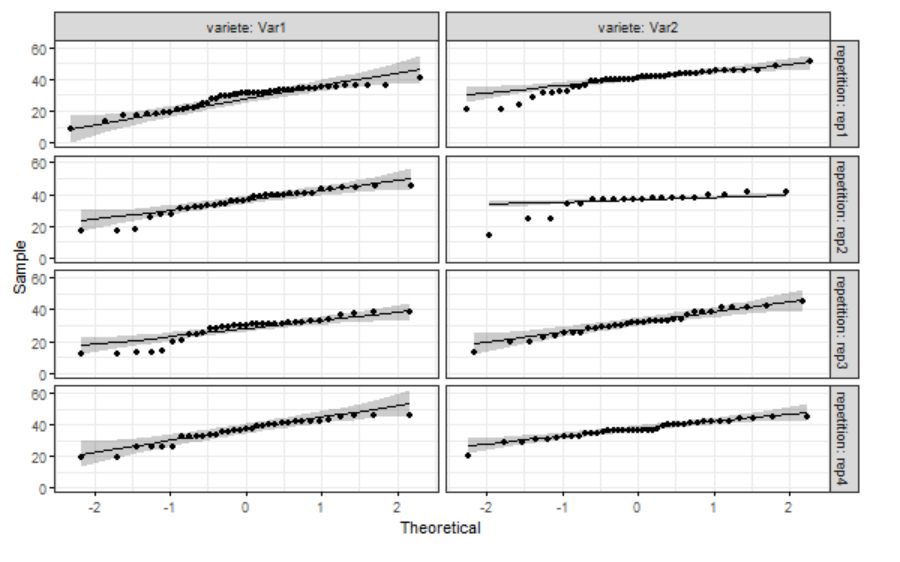
\includegraphics[width=0.85\textwidth]{figures/qqplot_normalite.png}
  \caption{QQ-plots de la hauteur par répétition et variété.}
  \label{fig:qqplot}
\end{figure}

\subsection*{Homogénéité des variances}
Le test de Levene (centré sur la médiane) a été appliqué séparément à chaque répétition afin d’évaluer l’hypothèse d’homogénéité des variances entre les groupes définis par les facteurs terreau et variété.
Les résultats indiquent que l’hypothèse d’égalité des variances n’est pas rejetée pour l’ensemble des répétitions :
rep1 (p = 0,727), rep2 (p = 0,797), rep3 (p = 0,502) et rep4 (p = 0,078).

Ainsi, pour chacune des répétitions, aucune hétéroscédasticité significative n’est détectée au seuil de 5\%. Bien que la p-value associée à la répétition 4 soit relativement proche du seuil de significativité, elle demeure non significative. L’hypothèse d’homogénéité des variances peut donc être considérée comme raisonnablement satisfaite dans l’ensemble du dispositif expérimental.

\subsection*{Sphéricité}
L'hypothèse de sphéricité a été testée automatiquement via le test de Mauchly dans le cadre
de la fonction \texttt{anova\_test()} (package \textit{rstatix}). Les corrections de
Greenhouse–Geisser ont été appliquées lorsque nécessaire, garantissant un ajustement des
degrés de liberté intra-sujets pour éviter une inflation du risque de type~I.

\section{Résultats de l'ANOVA à mesures répétées}

\subsection*{Effets principaux}
\begin{itemize}[leftmargin=*, label=\textbullet]
  \item \textbf{Terreau :} non significatif ($p = 0{,}303$, ges $= 0{,}012$) — le type de
        terreau n'influence pas significativement la hauteur.
  \item \textbf{Variété :} significatif ($p = 5{,}6 \times 10^{-4}$, ges $= 0{,}068$) — la
        hauteur varie selon la variété.
  \item \textbf{Répétition :} significatif ($p = 2{,}92 \times 10^{-4}$, ges $= 0{,}145$) —
        la hauteur évolue au fil des répétitions.
\end{itemize}

\subsection*{Interactions}
\begin{itemize}[leftmargin=*, label=\textbullet]
  \item \textbf{Variété $\times$ répétition :} significative ($p = 9{,}62 \times 10^{-5}$,
        ges $= 0{,}162$) — la différence entre variétés dépend du moment de mesure.
  \item \textbf{Terreau $\times$ variété, terreau $\times$ répétition, terreau $\times$
        variété $\times$ répétition :} non significatives ($p > 0{,}05$) — pas d'effet
        combiné notable impliquant le terreau.
\end{itemize}

Le temps (répétitions) et la variété influencent la croissance, tandis que le terreau seul
n'a pas d'effet majeur. L'interaction variété $\times$ répétition suggère que certaines
variétés croissent différemment selon les moments de mesure.

\section{Analyse post-hoc}

L'ANOVA globale indique l'existence d'une différence, sans préciser quels niveaux diffèrent.
Des comparaisons par paires (\texttt{pairwise\_t\_test}) avec correction Bonferroni ont donc
été réalisées par combinaison répétition $\times$ terreau pour identifier les variétés
statistiquement différentes.

Les résultats montrent que :
\begin{itemize}[leftmargin=*, label=\textbullet]
  \item \textbf{À rep1 :} pour tous les types de terreau (An, Ca, Ma), la différence entre
        Var1 et Var2 est significative (p-values Bonferroni : An $= 0{,}0074$, Ca et Ma
        $= 2{,}25 \times 10^{-5}$). Var2 est significativement plus haute que Var1 à rep1.
  \item \textbf{À rep2–rep4 :} aucune différence significative entre Var1 et Var2 pour aucun
        terreau ($p_{\text{adj}} > 0{,}05$). À partir de rep2, les hauteurs des deux variétés
        se rapprochent : la différence initiale disparaît.
\end{itemize}

L'effet de la variété est donc fort en début d'expérience (rep1) et s'estompe au fil des
répétitions, ce qui correspond bien à l'interaction significative variété $\times$ répétition.
Le type de terreau n'influence pas la différence entre Var1 et Var2.

\section{Modèle linéaire mixte}

Lorsque les données présentent des mesures répétées sur les mêmes unités statistiques,
l’ANOVA à mesures répétées classique peut devenir contraignante, notamment en cas de
déséquilibre du plan expérimental, de valeurs manquantes ou de structures de corrélation
complexes entre mesures successives. Dans ce contexte, les modèles linéaires mixtes (Linear
Mixed Models, LMM) constituent une alternative plus flexible et plus robuste.

Le principe du LMM consiste à combiner des \textit{effets fixes}, qui représentent l’influence
moyenne des facteurs expérimentaux (terreau, variété, répétition et leurs interactions), et
des \textit{effets aléatoires}, qui permettent de modéliser l’hétérogénéité individuelle entre
les sujets (plants). Cette approche permet de tenir compte explicitement de la corrélation
entre les mesures répétées effectuées sur un même individu, tout en conservant une
interprétation classique des effets des facteurs.

Dans ce travail, un modèle linéaire mixte avec intercept aléatoire par sujet a été ajusté afin
de capturer la variabilité inter-individuelle non expliquée par les facteurs observés. Le
modèle s’écrit :

\[
  \text{hauteur}_{ijk} = \mu + \alpha_i + \beta_j + \gamma_k + (\alpha\beta)_{ij} +
  (\alpha\gamma)_{ik} + (\beta\gamma)_{jk} + (\alpha\beta\gamma)_{ijk} + u_s + \varepsilon_{ijk},
\]

où $\mu$ représente la moyenne générale, $\alpha_i$, $\beta_j$ et $\gamma_k$ désignent
respectivement les effets fixes du type de terreau, de la variété et de la répétition, les
termes d’interaction traduisent les effets combinés des facteurs, $u_s$ correspond à l’effet
aléatoire associé au sujet $s$, supposé suivre une loi normale centrée
$u_s \sim \mathcal{N}(0, \sigma_u^2)$, et $\varepsilon_{ijk}$ désigne l’erreur résiduelle,
supposée suivre une loi normale centrée $\varepsilon_{ijk} \sim \mathcal{N}(0, \sigma^2)$.

L’intérêt principal de ce modèle est de fournir des tests d’effets fixes comparables à ceux de
l’ANOVA à mesures répétées, tout en offrant une meilleure prise en compte de la structure de
dépendance des données et une plus grande robustesse face aux déséquilibres du plan
expérimental.

\subsection*{Effets principaux}
\begin{itemize}[leftmargin=*, label=\textbullet]
  \item \textbf{Terreau :} $F(2, 258) = 0{,}062$, $p = 0{,}94$ — non significatif.
  \item \textbf{Variété :} $F(1, 258) = 14{,}14$, $p = 0{,}00021$ — hautement significatif.
  \item \textbf{Répétition :} $F(3, 258) = 9{,}70$, $p = 4{,}36 \times 10^{-6}$ — hautement
        significatif.
\end{itemize}

\subsection*{Interactions}
\begin{itemize}[leftmargin=*, label=\textbullet]
  \item \textbf{Variété $\times$ répétition :} $F(3, 258) = 9{,}88$, $p = 3{,}44 \times
        10^{-6}$ — significatif ; les trajectoires de croissance diffèrent selon la variété
        au fil du temps.
  \item \textbf{Terreau $\times$ variété, terreau $\times$ répétition, terreau $\times$
        variété $\times$ répétition :} $p > 0{,}88$ — non significatives.
\end{itemize}

Le LMM confirme les conclusions de l'ANOVA classique tout en offrant une approche robuste
face aux données déséquilibrées et aux valeurs manquantes.

% ============================================================
\chapter*{Conclusion et discussion}
\addcontentsline{toc}{chapter}{Conclusion et discussion}
% ============================================================

L'analyse descriptive met en évidence l'ordre de grandeur et la dispersion des hauteurs
observées. Les comparaisons bivariées et les profils moyens suggèrent des différences de
croissance selon la variété, avec des trajectoires temporelles non parallèles, tandis que
l'effet du terreau apparaît visuellement plus modéré. L'ACP révèle une hétérogénéité entre
répétitions, motivant l'usage d'une ANOVA à mesures répétées.

L'ANOVA à mesures répétées et le modèle linéaire mixte convergent vers les mêmes
conclusions : la variété et la répétition (temps) influencent significativement la hauteur
des plantes ; l'interaction variété $\times$ répétition est significative ; le type de
terreau n'a pas d'effet significatif, ni seul ni en interaction. Les tests post-hoc avec
correction Bonferroni confirment que la différence entre variétés est forte à rep1 et
s'efface à partir de rep2.

Ces résultats suggèrent que la croissance est majoritairement déterminée par la génétique de
la plante (variété) et le moment de mesure, et non par le substrat utilisé (terreau) dans
les conditions expérimentales étudiées.

\subsection*{Limites de l'étude}
La présence de valeurs manquantes (86 observations) et les faibles effectifs par cellule
limitent la puissance des tests. Par ailleurs, l'expérimentation se limite à quatre
répétitions et à un contexte spécifique, ce qui restreint la généralisation des résultats.

\subsection*{Perspectives}
Des études futures pourraient inclure un plus grand nombre de sujets, d'autres types de
terreau et des mesures à des intervalles plus fins afin de mieux caractériser les trajectoires
de croissance. L'utilisation de modèles non linéaires ou de courbes de croissance mixtes
pourrait également apporter des informations complémentaires.

% ============================================================
%  RÉFÉRENCES
% ============================================================
\clearpage

\pagenumbering{roman}
\setcounter{page}{5}

\chapter*{Références}
\addcontentsline{toc}{chapter}{Références}

American Journal of Reproductive Nutrition and Health. (2023). 
\textit{Application de l’ANOVA dans des études expérimentales}. 
\url{https://journalajrnh.com/index.php/AJRNH/article/view/194/402}

\vspace{0.3cm}

DataNoVIA. (2024). 
\textit{ANOVA mixte dans R : hypothèses et mise en œuvre}. 
\url{https://www.datanovia.com/en/fr/lessons/anova-mixte-dans-r/}

\vspace{0.3cm}

Liang, X., et al. (2024). 
\textit{Application des modèles à mesures répétées dans l’analyse de données expérimentales}. 
\textit{Heliyon}. 
\url{https://www.sciencedirect.com/science/article/pii/S2405844024075327}

\vspace{0.3cm}

NumiQO. (2023). 
\textit{ANOVA avec mesures répétées : tutoriel méthodologique}. 
\url{https://numiqo.fr/tutorial/anova-with-repeated-measures}

\vspace{0.3cm}

Park, E., Cho, M., \& Ki, C.-S. (2009). 
Correct use of repeated measures analysis of variance. 
\textit{Korean Journal of Laboratory Medicine, 29}(1), 1--9. 
\url{https://pubmed.ncbi.nlm.nih.gov/19262072/}

\vspace{0.3cm}

Xu, R., et al. (2025). 
\textit{Repeated measures design in agronomy experiments}. 
\textit{Agronomy, 15}(5), 1055. 
\url{https://www.mdpi.com/2073-4395/15/5/1055}

\end{document}